\section{KaioKen}

	\subsection{Descripción del Problema}
		Sea $n \in \mathds{N}$, $c: conj(lista(nat))$. El objetivo de este problema es encontrar la menor cantidad de listas necesarias que cumplan con las siguientes condiciones: 
		    \begin{itemize}
                \item ($ \forall l \in c$) tam($l$) = $n$
                \item ($ \forall l \in c$) ($ \forall i < n$) $l[i]$ = 1 $\vee$ $l[i]$ = 2
                \item ($ \forall i < n$) ($ \forall j < n$) $\exists$ ($l \in c$) $l[i] \neq l[j]$
            \end{itemize}
    Es decir, todas las listas deben tener tamaño igual a $n$, y sus elementos deben ser 1 o 2. Se trata de minimizar el cardinal del conjunto $c$ cumpliendo con las tres condiciones. 
    Por ejemplo:\\
    
      Para n = 4  \\
    \\

\begin{wrapfigure}{l}{3cm}
  \vspace{-41pt}
  \begin{center}
    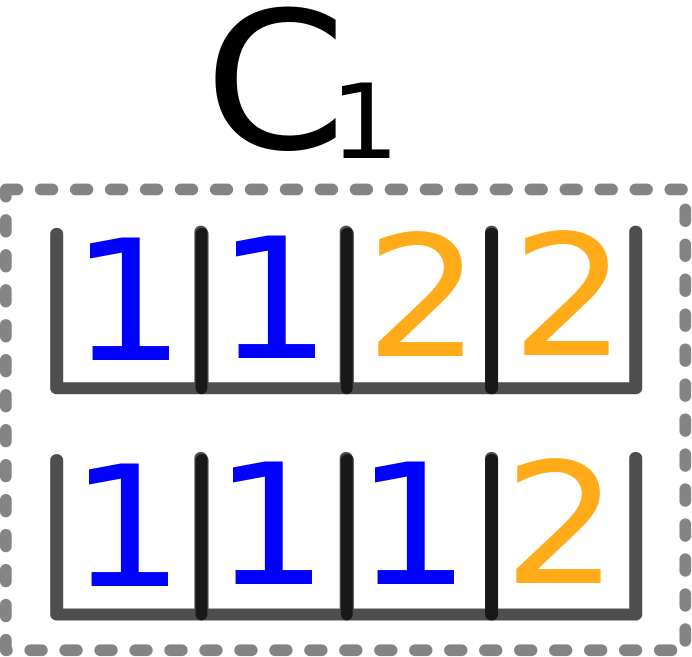
\includegraphics[width=2cm]{graficos/c1.png}
  \end{center}
\end{wrapfigure}

 El conjunto $C_{1}$ no es una solución válida ya que no cumple con la tercera condición. Para $i$=0, $j$=1, no existe una lista $l$ donde $l[i] \neq l[j]$.
\\
\\
\\

\begin{wrapfigure}{l}{3cm}
  \vspace{-41pt}
  \begin{center}
    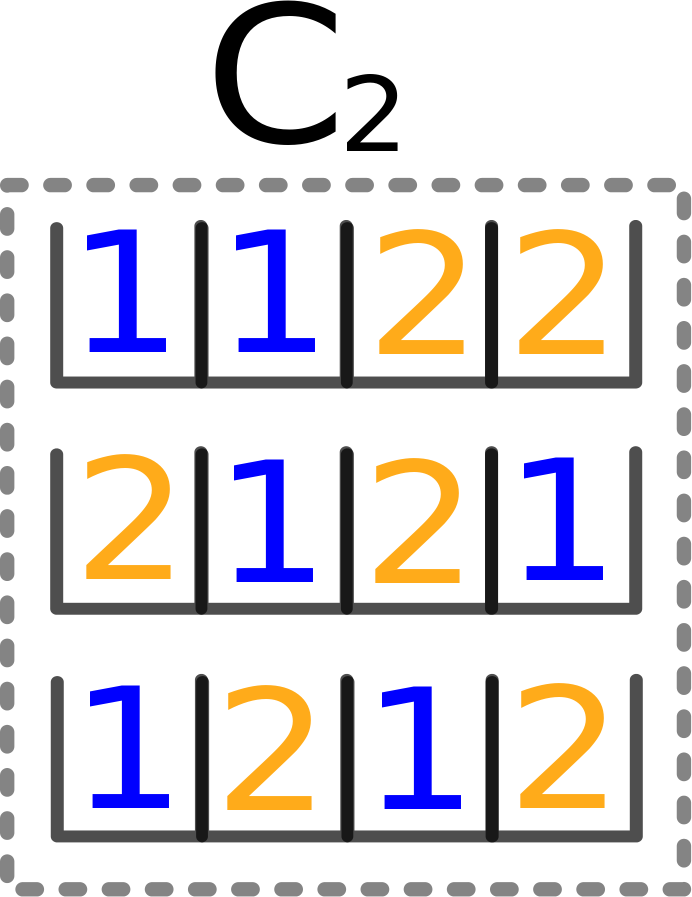
\includegraphics[width=2cm]{graficos/c2.png}
  \end{center}
\end{wrapfigure}

 El conjunto $C_{2}$ tampoco es una respuesta correcta ya que omitiendo alguna de las listas el conjunto sigue cumpliendo con las tres condiciones nombradas anteriormente. \\
 \\
 \\

{\begin{tabular}{ccc}
   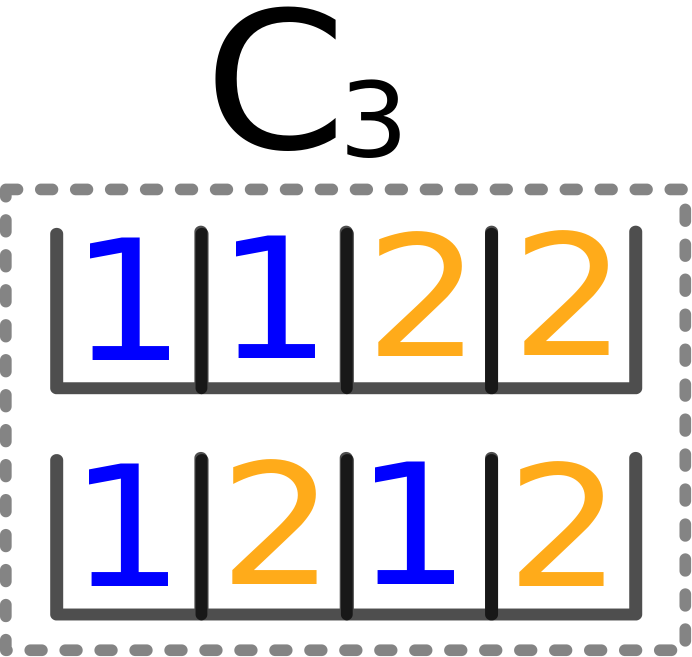
\includegraphics[height=2cm]{graficos/c3.png} & 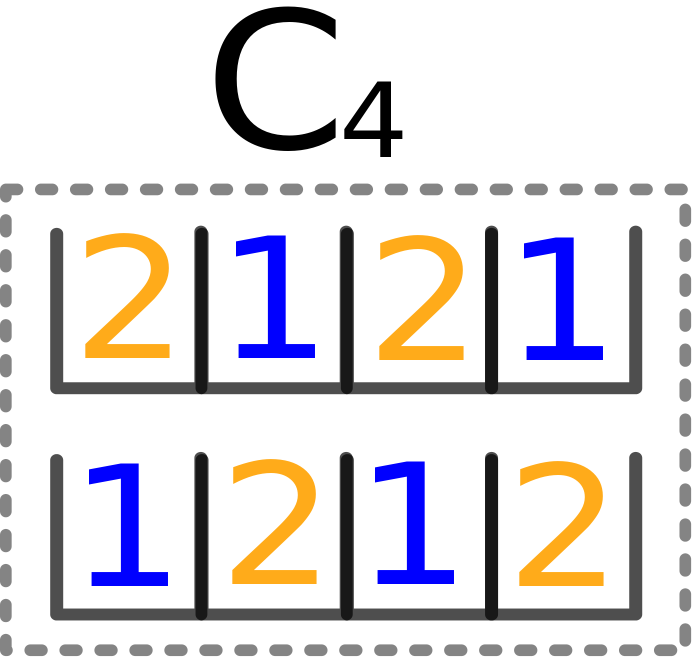
\includegraphics[height=2cm]{graficos/c4.png} & 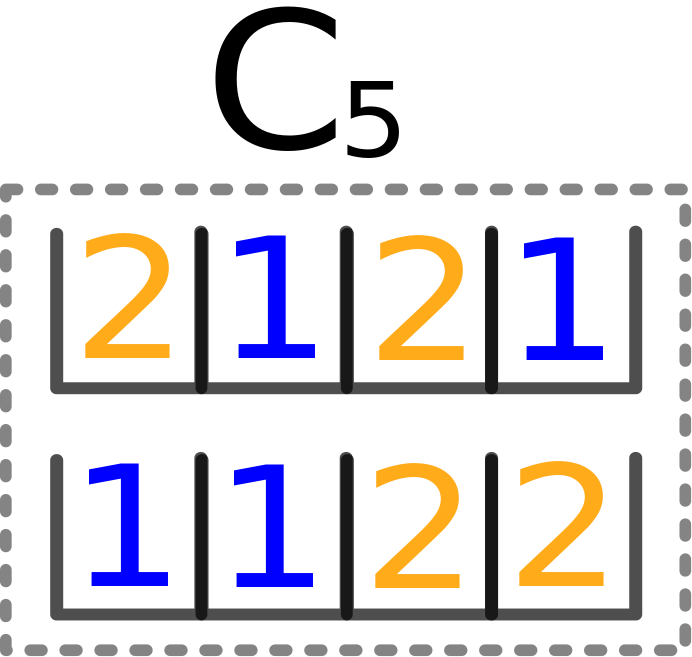
\includegraphics[height=2cm]{graficos/c5.png} \\
   \\

\end{tabular}}

  Los conjuntos $C_{3}$, $C_{4}$ y $C_{5}$ son respuestas válidas. 




    \subsection{Desarrollo}


    \subsection{Complejidad}

    \begin{algoritmo}{kaioken}{int n}{int}

  \tipo{int} $cantMinPeleas \gets \lceil log_{2}(n) \rceil$ \com*{O(1)}
  \tipo{int} $equipo$ \com*{O(1)}

  \For(\com*{O($log_{2}(n)$)}){($i$ = 1; $i \leq cantMinPeleas$; $i$++)}{
    $equipo \gets 1$ \com*{O(1)}
    \For(\com*{O($n/2^{i-1}$)}){($h$ = 1; $h \leq n$; $h$ = $h + 2^{i-1}$)}{
      \For(\com*{O($2^{i-1}$)}){($k$ = 0; ($k < 2^{i-1}$) $\&$ ($h+k \leq n$); $k$++)}{
        escribir($equipo$) \com*{O(1)}
      }
        \eIf(\com*[f]{O(1)}){$equipo == 1$}{
          $equipo \gets 2$ \;
        }{
          $equipo \gets 1$ \;
        }
    }
  }


\end{algoritmo}

El segundo ciclo junto con el tercer ciclo tienen complejidad O($n$), ya que se multiplica O($n/2^{i-1}$) por O($2^{i-1}$). Entre los dos ciclos se recorren todos los guerreros una vez. El segundo recorre por grupos de guerreros que van a pertenecer al mismo equipo y el segundo de ellos le asigna a cada guerrero de un grupo el número de equipo correspondiente. 

Por ejemplo, para $n$=8, el ciclo número dos recorre como indican las flechas rojas para la pelea 1, 2 y 3 respectivamente. El tercer ciclo, avanza por los enemigos entre las flechas rojas. Se puede observar que el vector se recorre una sola vez para cada pelea. 


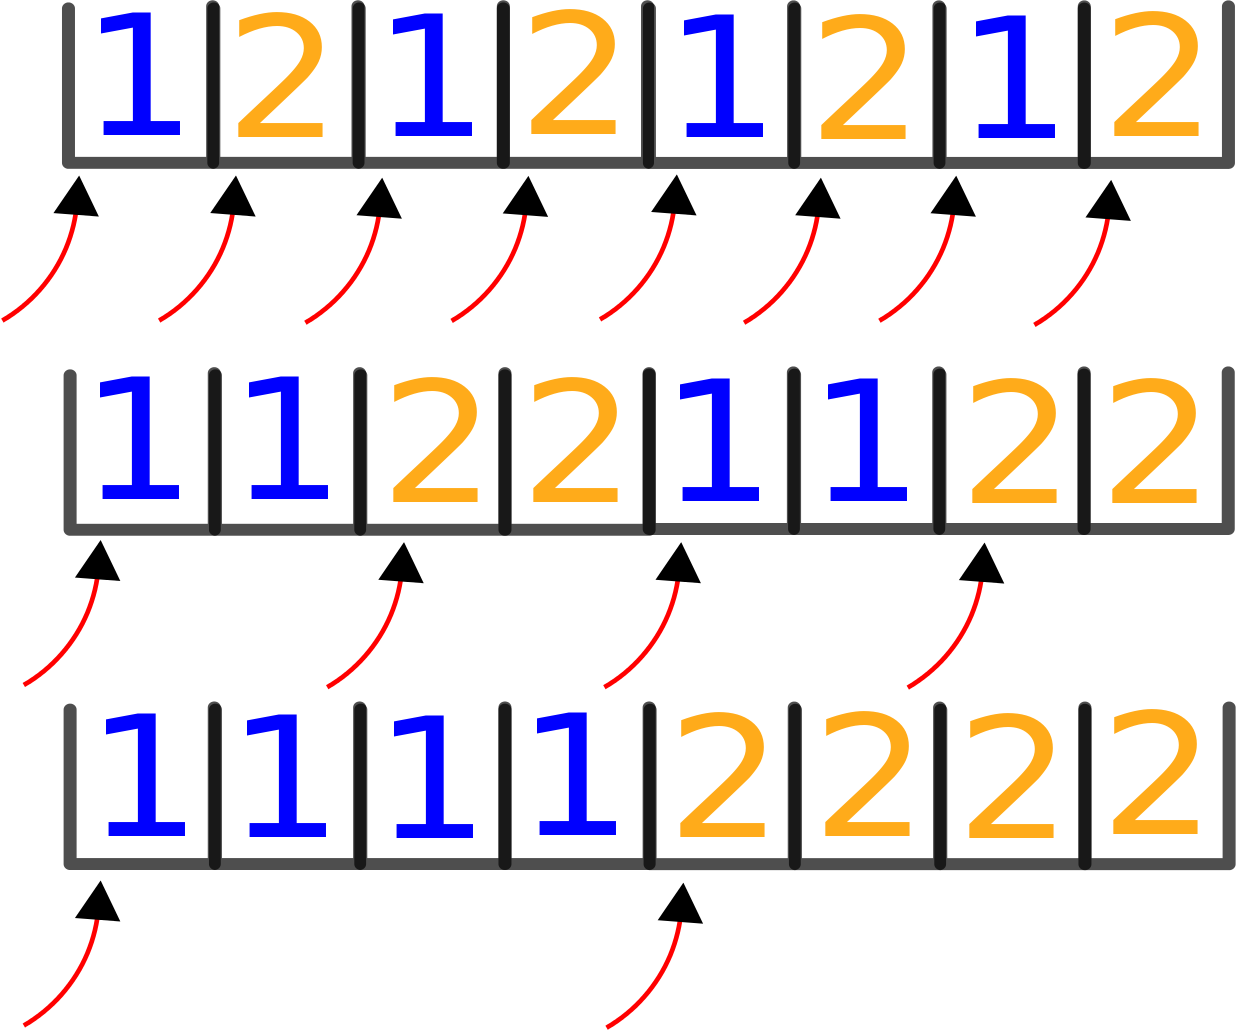
\includegraphics[height=4cm]{graficos/ciclo.png}


    \subsection{Código}


    \subsection{Experimentación}
		El objetivo de este experimento fue extraer conclusiones acerca de la variación en el tiempo de cómputo requerido por el algoritmo para distintos valores de $n$, con el fin de determinar su complejidad. 
		Para realizar las mediciones se  utilizaron las funciones provistas a tal efecto por la cátedra. Además, para evitar posibles errores en las mismas, cada una se repitió 7 veces, considerando luego el promedio entre los valores obtenidos. En este caso, se consideraron valores de $n$ entre 10000 y 300000.

    Para evaluar la complejidad del algoritmo, se graficó la curva $n \times log_{2}n / 13000000$.

      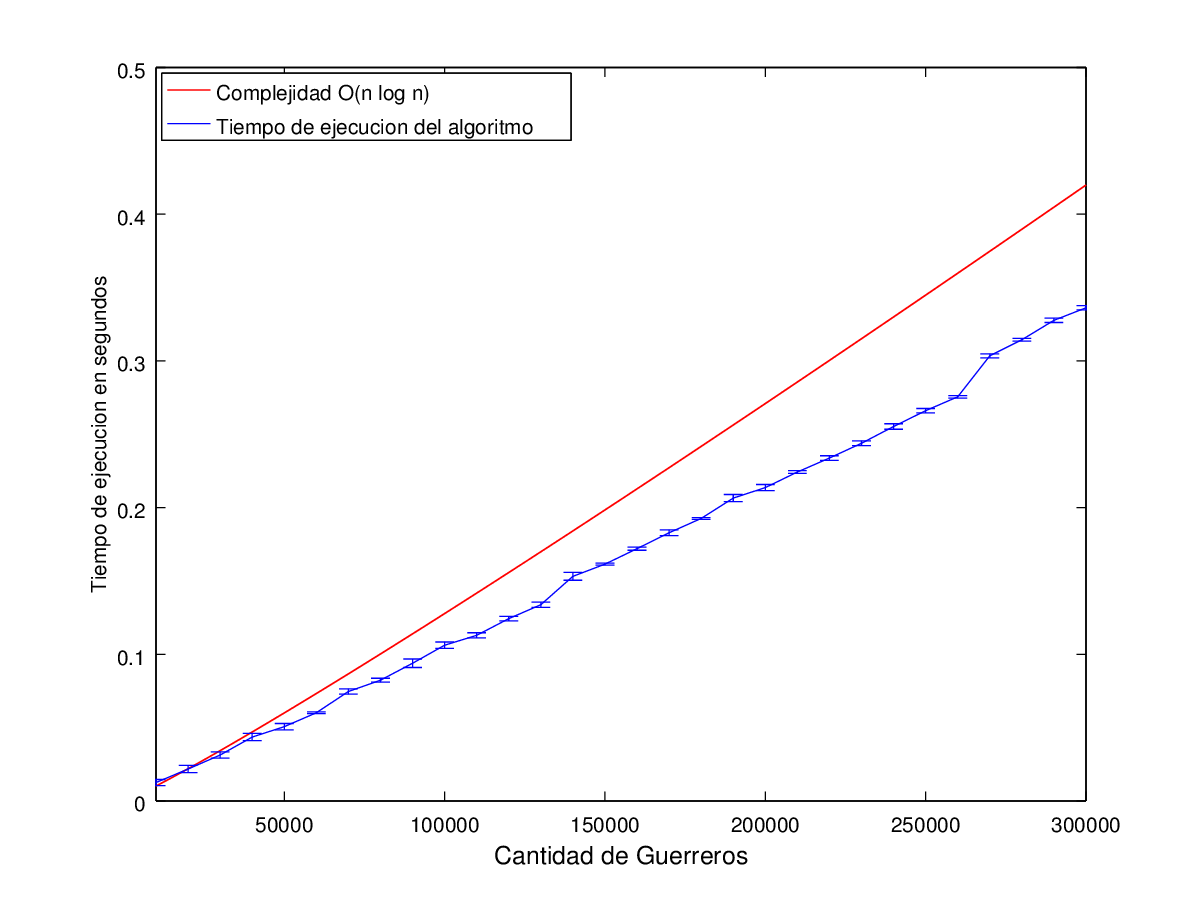
\includegraphics[height=11cm]{graficos/kaioken-exp.png}



		\subsubsection*{Conclusión}
			Se puede observar en el gráfico que la curva $n \times log_{2}n / 13000000$ está por encima de la curva que forman las mediciones del tiempo de ejecución del programa. Por lo tanto, se demuestra empiricamente que la complejidad del programa es O($n \times log_{2}n$)
